\label{sec:schritte}

\section{Installation des Betriebsystems}
\label{sec:stepsinstall}
Dieses Kapitel beschreibt die Installation und Einrichtung des Betriebsystems auf einer SD-Karte bis das Raspberry gestartet werden kann und mit Maus und Tastatur mit einer normalen Desktop-Oberfläche verwendet werden kann. (Teile der Anleitung für Windows übernommen von \cite{install}.)

\begin{itemize}
	\item {Erster Schritt ist der Download des aktuellsten raspbian Images.\\
%		Auf \url{https://www.raspberrypi.org/downloads/raspbian/} gibt es den Abschnitt \begin{em}Raspbian\end{em} mit einem Punkt \begin{em}Raspbian Wheezy\end{em}. 
		Auf \url{https://www.raspberrypi.org/downloads/raspbian/} gibt es den Abschnitt \begin{em}Raspbian\end{em} mit einem Punkt \begin{em}Raspbian Jessie\end{em}. 
		Diese ZIP-Datei muss heruntergeladen werden.
		(ca. 1,3 Gigabyte)
%		(Hinweis: Die Version \begin{em}Raspbian Jessie\end{em} mit \begin{em}Release date: 2015-11-21\end{em} wurde auch getestet, jedoch funktionierte in dieser Version der Internet-Browser nicht richtig.)
		}
	\item {Hinweis: Zur Zeit lautet die Datei \lstinline|2016-03-18-raspbian-jessie.zip|.
		In unregelmäßigen Abständen wird das raspbian Image aktualisiert.
		Es ist daher möglich, dass diese Schritt-für-Schritt Anleitung bei zukünftigen Versionen nicht mehr problemlos funktioniert.
		Bitte in einem solchen Fall um eine Info an \verb|edv@bfkdo-tulln.at|, damit die Anleitung aktualisiert werden kann.}
	\item {Nach dem Download muss die ZIP-Datei entpackt werden. In dieser befindet sich eine IMG-Datei, welche das Betriebssystem behinhaltet.}
	\item {Windows-Benutzer benötigen zum Überspielen des Images auf die SD-Karte das Tool Win32DiskImager.\\
		Dieses kann unter \url{http://sourceforge.net/projects/win32diskimager/} heruntergeladen werden. 
		Nach dem Download muss die ZIP-Datei entpackt werden.
		}
	\item {Linux-Benutzer können das Image mit \lstinline|dd| auf die SD-Karte kopieren. Dieses ist in den meisten Distributionen bereits installiert.
		}
	\item {Windows-Benutzer öffnen die soeben heruntergeladene Win32DiskImager.exe. Im Feld Image File muss man nun das heruntergelaene Raspbian Image einbinden. 
		Im nebenstehenden Feld Device muss man den Laufwerksbuchstaben auswählen auf welches das Image Installiert werden soll. 
		Wenn man sichergestellt hat, dass beide Angaben korrekt sind klickt man auf Write und das Image wird auf die SD-Karte geschrieben.
		}
	\item {Linux-Benutzer sollten einen Terminal mit root-Rechten öffnen. 
		Mit \lstinline|fdisk -l| oder \lstinline|lsblk| können alle verfügbaren Speichermedien aufgelistet werden. Darunter muss die SD-Karte gefunden werden.
		Typischerweise ist es \lstinline|/dev/sdb|, \lstinline|/dev/sdc|, etc.
		Auch \lstinline|dmesg| ist hilfreich, um die eben erst angelossene Karte zu finden. 
		Mit \lstinline|mount| werden die aktuell eingebundenen Laufwerke aufgelistet und 
		die SD-Karte ggf. mit \lstinline|umount /dev/sdb*| (je nachdem als welches Device die Karte erkannt wurde) entfernt.
		Mit \lstinline|dd bs=8M if=/pfad/zu/datei/2016-03-18-raspbian-jessie.img of=/dev/sdb| kann das Image auf die SD-Karte kopiert werden.
		Das dauert einige Zeit und es gibt keine Fortschrittsanzeige.
		\textbf{Achtung:} Wichtig ist dabei, unbedingt das richtige Device (\lstinline|/dev/sdb|, \lstinline|/dev/sdc|, etc.) anzugeben, 
		da sonst eventuell die lokale Festplatte des PCs überschrieben wird!
		}
	\item {Als nächstes kann die SD-Karte ins RaspberryPi eingesetzt werden. Dann Maus, Tastatur, Bildschirm und Netzwerk angeschlossen werden. 
		Als letztes wird die Stromversorgung angeschlossen und das RaspberryPi startet automatisch.
		}
	\item {Beim Start wird links oben eine Himbeere angezeigt und es laufen verschiedene Textnachrichten durch das Bild. 
		Das RaspberryPi sollte direkt mit einer grafischen Benutzeroberfläche starten und als Hintergrund eine Himbeere (ähnlich wie in \reffig{rpidesktop}) anzeigen.
		}
	\item {Um das System weiter einzurichten, muss nun ein Terminal geöffnet werden.
		Das Symbol dafür befindet sich links oben (siehe \reffig{rpiterminal}).
		Dann wird folgender Befehl eingegeben und mit \lstinline|Enter| bestätigt:\\
		\lstinline|setxkbmap de|\\
		Danach wird folgender Befehl eingegeben und erneut mit \lstinline|Enter| bestätigt:\\
		\lstinline|sudo raspi-config|
		}
	\item {Es wird ein Menü ähnlich wie in \reffig{menu} angezeigt, mit den Optionen zur Einrichtung des Betriebsystems. 
		(Im Menü wird mit den Cursortasten navigiert, mit Tabulator kann zu Select, Finish, etc. gesprungen und mit Enter betätigt werden. Optionen werden mit der Leertaste ausgewählt.
		\begin{itemize}
		\item {Zuerst sollte das Dateisystem auf die komplette Größe der SD-Karte erweitert werden
			(Eintrag \lstinline|Expand Filesystem|). Die tatsächliche Vergrößerung wird beim nächsten Neustart durchgefürt.}
		\item {Ebenso sollte das Default-Passwort geändert werden (Eintrag \lstinline|Change User Password|). Dieses Passwort wird später noch benötigt.
			(Hinweis: Bei der Eingabe des Passwortes wird nichts angezeigt. Auch keine \lstinline|*|-Zeichen.)}
%		\item {Unter \lstinline|Enable Boot to Desktop/Scratch| wird die Option \lstinline|Desktop Log in as user pi at the graphical desktop| ausgewählt. 
%			Diese Option startet automatisch eine grafische Benutzeroberfläche.}
%		\item {Unter \lstinline|Internationalisation Options| $\rightarrow$ \lstinline|Change Locale| wird die Option \lstinline|de_AT.UTF-8 UTF-8| aktiviert und auf der 
%			nächsten Seite als Default ausgewählt. Damit wird die Sprache von Englisch auf Deutsch umgestellt.}
%		\item {Unter \lstinline|Internationalisation Options| $\rightarrow$ \lstinline|Change Timezone| kann die Zeitzone auf \lstinline|Europe| $\rightarrow$ \lstinline|Vienna| eingestellt werden.}
%		\item {Unter \lstinline|Internationalisation Options| $\rightarrow$ \lstinline|Change Keyboard Layout| kann die Tastaturbelegung auf 
%			Deutsch eingestellt werden. Dazu muss ausgewählt werden: \lstinline|Generic 105-key (Intl) PC| $\rightarrow$ \lstinline|Other| $\rightarrow$ \lstinline|German (Austria)| $\rightarrow$ \lstinline|German (Austria) - German (Austria, eliminate dead keys)| $\rightarrow$ \lstinline|The default for the keyboard layout| $\rightarrow$ \lstinline|No compose key| $\rightarrow$ \lstinline|No|.}
%		\item {Unter \lstinline|Advanced Options| $\rightarrow$ \lstinline|SSH| sollte \lstinline|enable| gewählt werden, damit das RaspberryPi über Netzwerk erreichbar ist.}
		\item {Mit \lstinline|Finish| $\rightarrow$ \lstinline|No| wird die Einrichtung abgeschlossen.}
		\end{itemize}
		}
	\item {Damit das RaspberryPi über das Netzwerk erreicht werden kann, ist es sinnvoll es am DHCP-Server (z.b. dem Router) als statisches Lease \cite{lease} einzutragen.
		Dabei wird vom DHCP-Server immer wieder die gleiche IP für das RaspberryPi vergeben und es kann mit dieser fixen IP von einem anderen Rechner im Netzwerk erreicht werden.
		Dieser Eintrag kann meist am Webinterface des Routers vorgenommen werden.
		Um die MAC-Adresse des RaspberryPi herauszufinden, muss auf der Konsole \lstinline|ifconfig eth0| eingegeben werden.
		(Die MAC-Adresse wird neben \lstinline|Hardware Adresse| ausgegeben.)
		}
	\item {Nachdem die MAC-Adresse zur gewünschten IP am Router eingetragen wurde, sollte das RaspberryPi mit dem Befehl \lstinline|sudo reboot| neu gestartet werden.
		}
	\item {Das RaspberryPi sollte nun erneut mit der grafischen Benutzeroberfläche starten.
		Die Installation und Einrichtung des Betriebsystems ist damit fertig.
		}
\end{itemize}

\begin{figure}[h!]
	\centering
		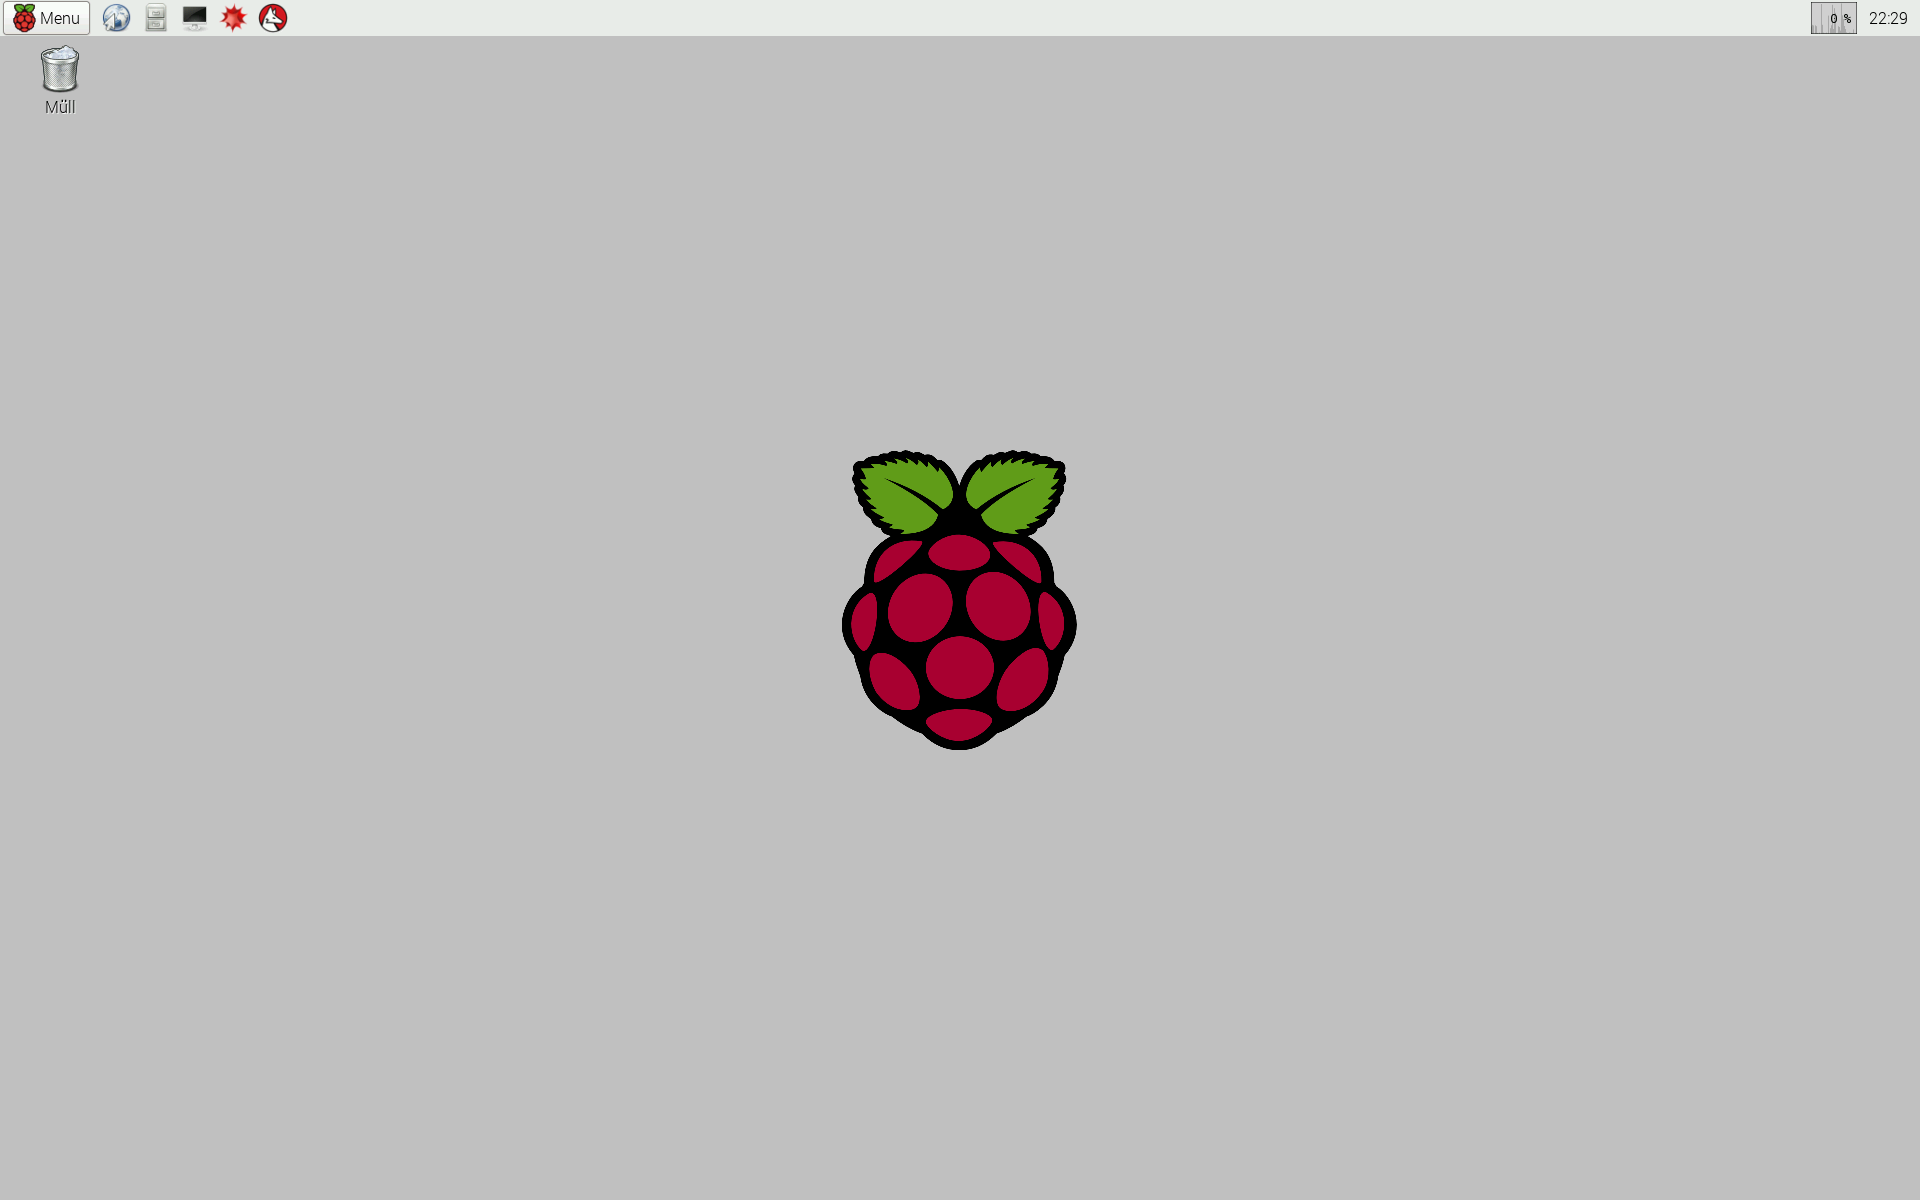
\includegraphics[width=0.8\textwidth]{./fotos/2015-02-08-222932_1920x1200_scrot.png}
	\caption{Desktop der grafischen Benutzeroberfläche am RaspberryPi}
	\label{fig:rpidesktop}
\end{figure}

\begin{figure}[h!]
	\centering
		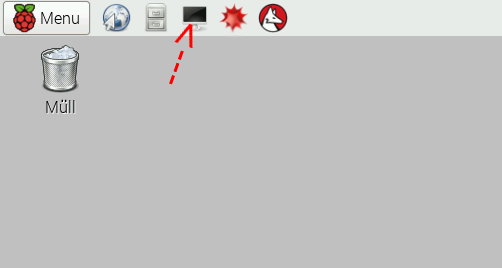
\includegraphics[width=0.8\textwidth]{./fotos/terminal.png}
	\caption{Symbol zum Start eines Terminal-Fensters}
	\label{fig:rpiterminal}
\end{figure}

\begin{figure}[h!]
	\centering
		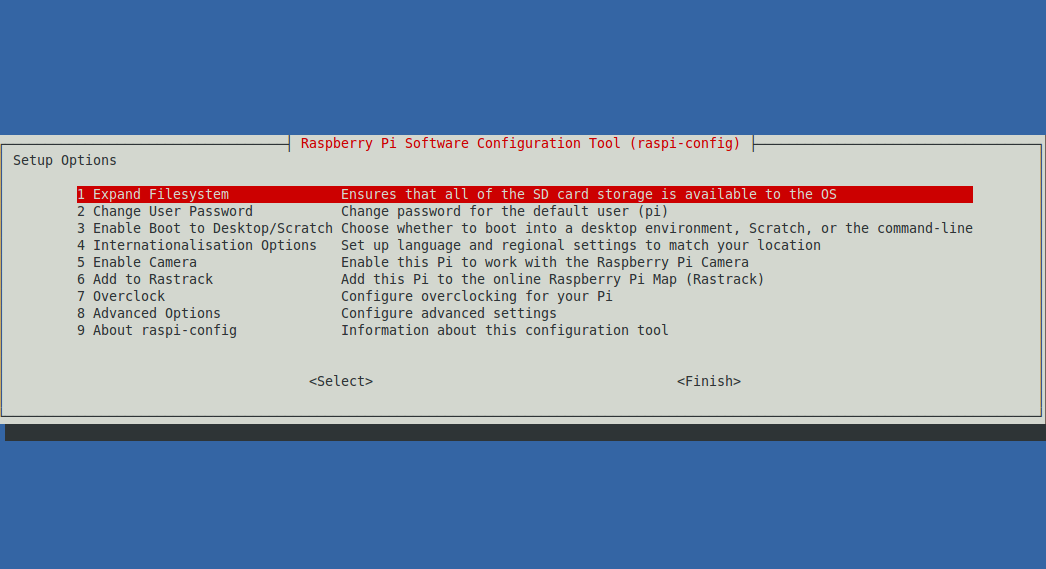
\includegraphics[width=0.9\textwidth]{./fotos/menu1.png}
	\caption{Menü zur Einrichtung des Betriebsystems}
	\label{fig:menu}
\end{figure}

\clearpage

\section{Einrichtung des Infoscreens}
\label{sec:stepssetup}
Für die weiteren Schritte werden keine Tastatur und Maus mehr am RaspberryPi benötigt. 
Sämtliche Schritte werden so beschrieben, dass sie über das Netzwerk von einem anderen Computer durchgeführt werden können.

\begin{itemize}
	\item {Windows-Benutzer benötigen zur Verbindung zum RaspberryPi das Tool PuTTY \cite{putty}.\\
		Dieses kann unter \url{http://www.chiark.greenend.org.uk/\~sgtatham/putty/download.html} heruntergeladen werden. 
		Es kann entweder die \lstinline|putty.exe| im Abschnitt \begin{em}For Windows on Intel x86\end{em} oder das Installationspakt im Abschnitt \begin{em}A Windows installer for everything except PuTTYtel\end{em} verwendet werden.
		}
	\item {Linux-Benutzer können den Befehl \lstinline|ssh| verwenden. Dieser ist in den meisten Distributionen bereits installiert.
		}
	\item {In PuTTY muss im Feld \lstinline|Host Name (or IP address)| die IP-Adresse des RaspberryPi angegeben werden. Mit Klick auf \lstinline|Open| wird die Verbindung hergestellt.
		Siehe auch \reffig{putty1} (in diesem Beispiel wäre die IP-Adresse \lstinline|10.34.17.227|).
		(Bei der ersten Verbindung wird ein \begin{em}PuTTY Security Alert\end{em} angezeigt. 
		Das ist der Fall, weil noch keine Verbindungsinformationen zum RaspberryPi gespeichert wurden. Dies muss mit \lstinline|Ja| bestätigt werden.)
		}
	\item {Bei \lstinline|login as:| wird der Username \lstinline|pi| eingegeben und mit \lstinline|Enter| bestätigt.
		Als Passwort muss das angegeben werden, welches im vorherigen Abschnitt (bei \lstinline|Change User Password|) gewählt wurde.
		(Hinweis: Bei der Eingabe des Passwortes wird nichts angezeigt. Auch keine \lstinline|*|-Zeichen.)\\
		Nach dem Erfolreichen Login wird \lstinline|pi@raspberrypi ~ $| angezeigt (ähnlich wie in \reffig{putty2}).
		}
	\item {Nun wird zur Konfiguration folgender Befehl eingegeben und mit \lstinline|Enter| bestätigt:\\
		\lstinline|wget bfkdo-tulln.at/is76/ -O s.sh; chmod +x s.sh; sudo ./s.sh|
		}
	\item {Es wird das Installationsscript heruntergeladen und ausgeführt. Die Ausgabe sollte so ähnlich aussehen:
		\begin{lstlisting}
###############################################
Installations-Script         Version 2016-05-09
###############################################
Infoscreen wird eingerichtet:
   Der Vorgang kann einige Minuten dauern, bitte um etwas Geduld!
- Zeitzone wurde eingerichtet.
- Systemzeit wurde aktualisiert.
- Sprache wurde eingerichtet.
- Tastaturlayout wurde eingerichtet.
- Software-Paketliste wurde aktualisiert.
- Paket "iceweasel" wurde installiert.
- Paket "unclutter" wurde installiert.
- Paket "x11-xserver-utils" wurde installiert.
- Paket "xmlstarlet" wurde installiert.
- Browser wurde in Autostart eingetragen.
- Firefox extension wurde heruntergeladen.
- Firefox extension wurde installiert.
- Browsereinstellungen wurden konfiguriert.
- Hintergrund wurde heruntergeladen.
- Einstellungen fuer Neustart gespeichert.
- Einstellungen fuer Bildschirm-Standby gespeichert.
Fertig.
###############################################
		\end{lstlisting}
		}
	\item {Danach wird das RaspberryPi mit dem Befehl \lstinline|sudo reboot| neu gestartet. 
		(Das RaspberryPi startet innerhalb maximal 5 Minuten auch automatisch neu, da der Internet-Browser noch nicht gestartet ist. 
		Es wird periodisch geprüft, ob der Internet-Browser läuft und ggf. ein Neustart durchgeführt.)}
	\item {Das RaspberryPi sollte automatisch den Internet-Browser starten und den Infoscreen anzeigen. Der Token muss auf der Admin-Seite des Infoscreens eingetragen werden.}
	\item {Falls noch eine Tastatur angeschlossen ist, kann die Seite mit \lstinline|F5| neu geladen werden.
		Andernfalls wird erneut eine Verbindung mit PuTTY hergestellt (siehe Punkte weiter oben) und das RaspberryPi mit dem Befehl \lstinline|sudo reboot| nochmals neu gestartet.
		}
	\item {Das RaspberryPi sollte wieder automatisch den Internet-Browser starten und den Infoscreen (dieses Mal mit den letzten Einsätzen) anzeigen.\\
		Der Infoscreen ist nun fertig eingerichtet.}
\end{itemize}

\begin{figure}[h!]
	\centering
		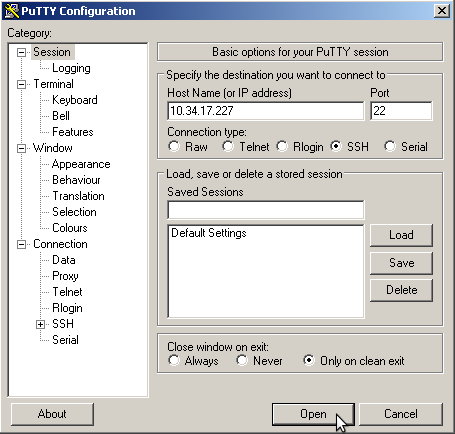
\includegraphics[width=0.6\textwidth]{./fotos/putty1.png}
	\caption{Verbindungseinstellungen mit PuTTY}
	\label{fig:putty1}
\end{figure}

\begin{figure}[h!]
	\centering
		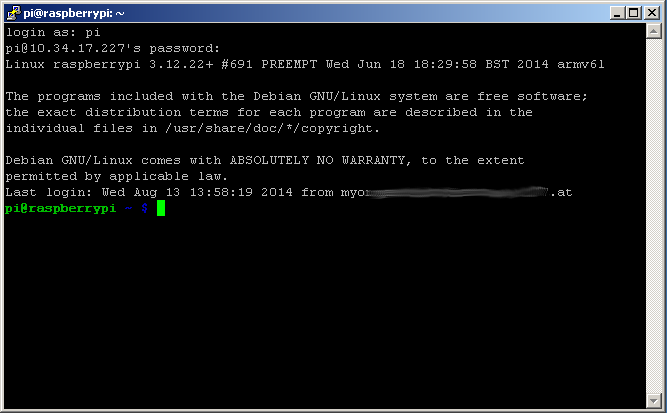
\includegraphics[width=0.8\textwidth]{./fotos/putty2.png}
	\caption{Verbindung mit PuTTY hergestellt}
	\label{fig:putty2}
\end{figure}



